\documentclass{standalone}
\usepackage{tikz}
\usetikzlibrary{patterns, positioning}
\usepackage[sfdefault]{ClearSans} %% option 'sfdefault' activates Clear Sans as the default text font
\usepackage[T1]{fontenc}

\begin{document}
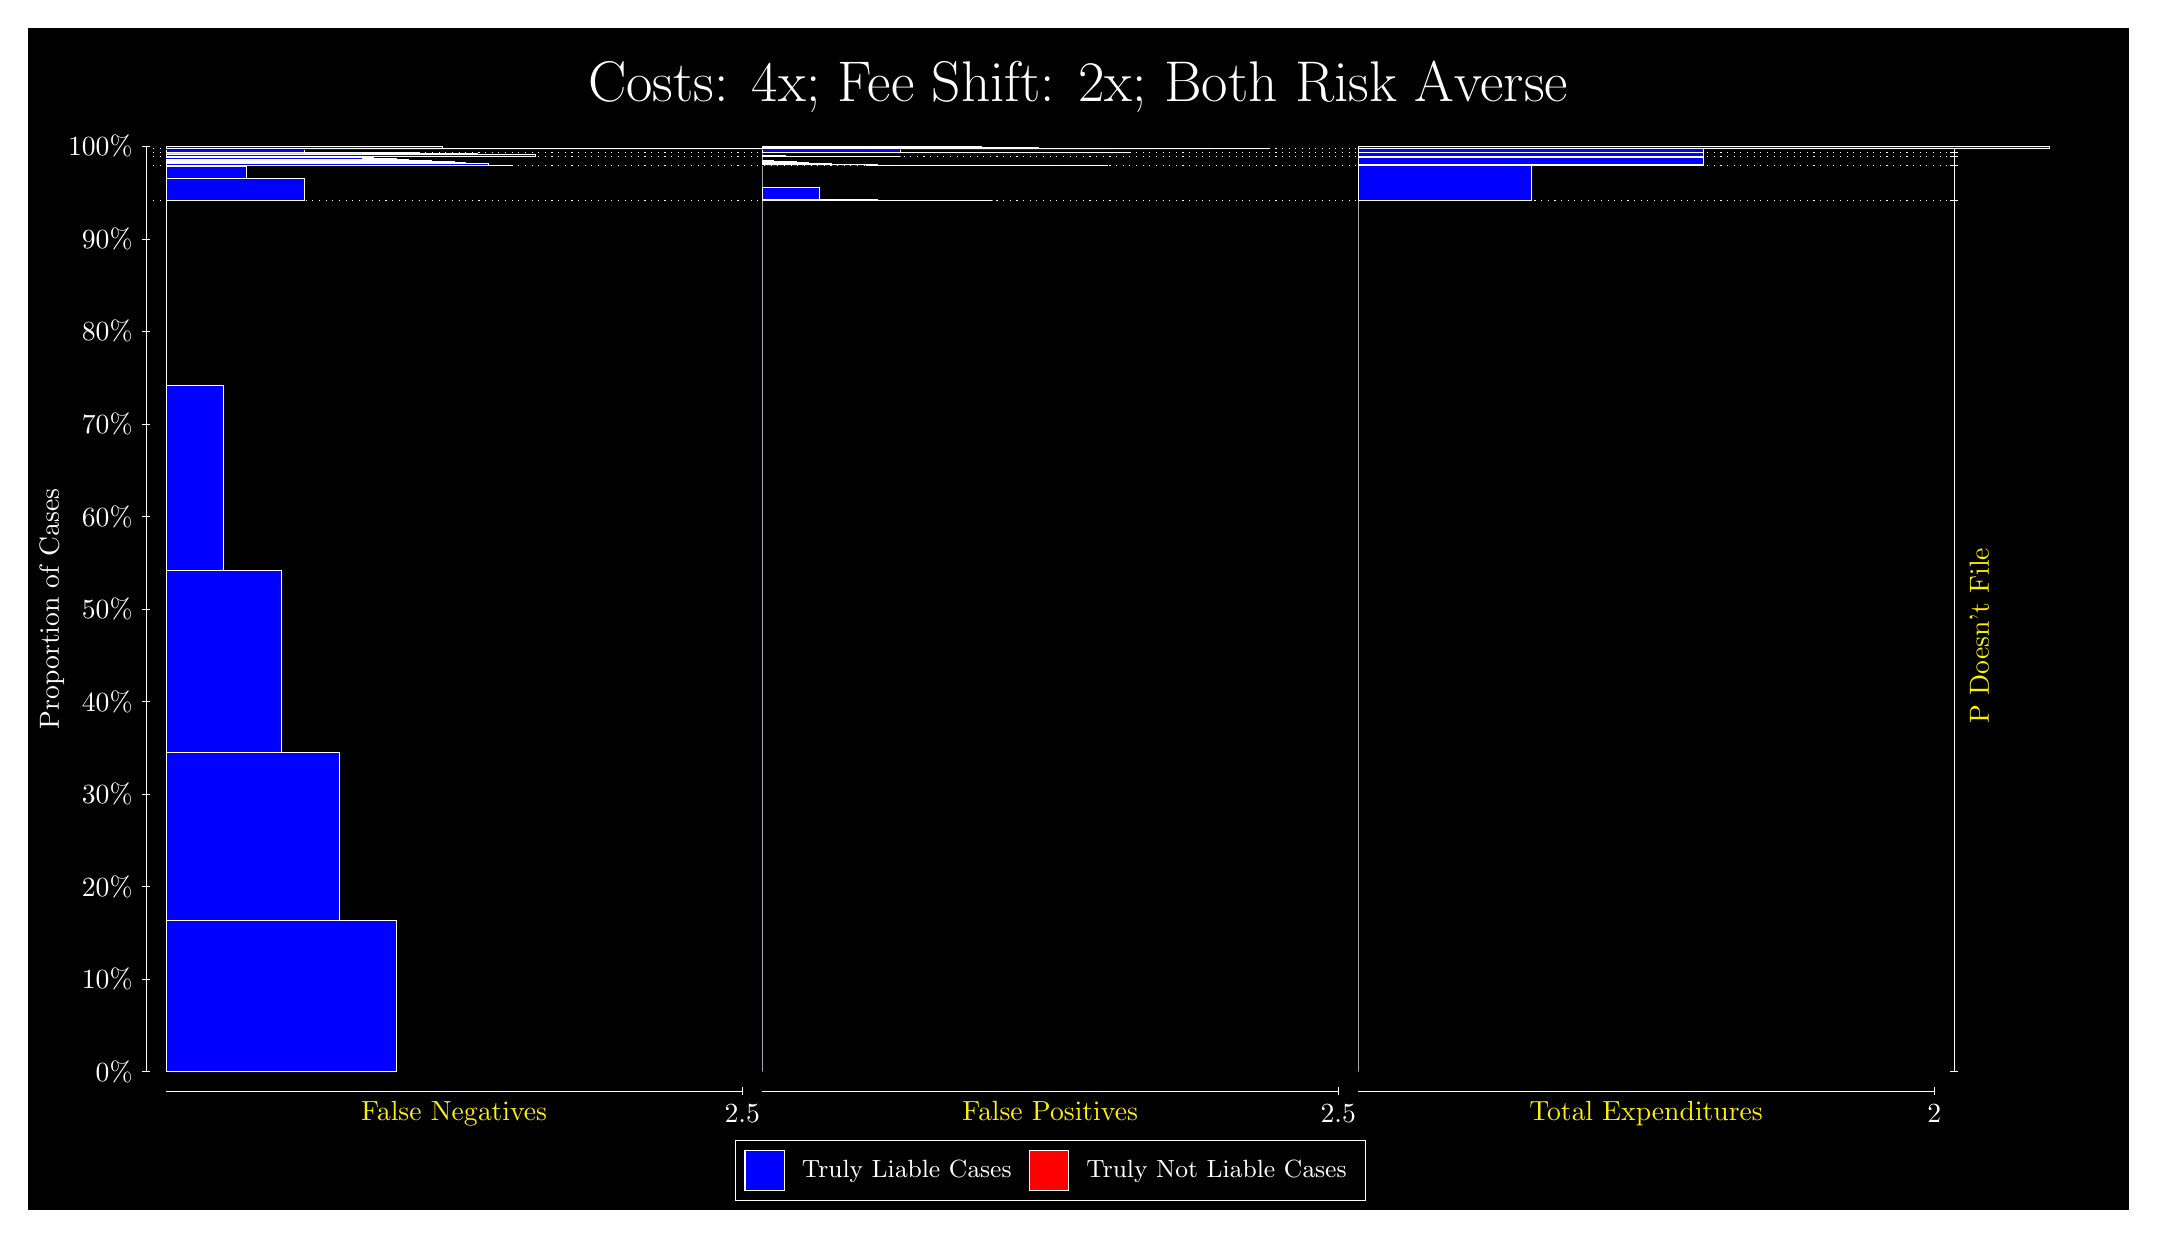
\begin{tikzpicture}
\draw[fill=black] (0,0) rectangle (26.667,15);
\draw[text=white] (0,13.5) rectangle (26.667,15) node[midway] {\huge Costs: 4x; Fee Shift: 2x; Both Risk Averse};
\draw[white, very thin] (1.5,1.75) -- (1.5,13.5);
\node[rotate=90, text=white, anchor=center] at (0.3, 7.625) {Proportion of Cases};
\draw[white, very thin] (1.45,1.75) -- (1.55,1.75);
\node[text=white, anchor=east] at (1.45, 1.75) {0\%};
\draw[white, very thin] (1.45,2.925) -- (1.55,2.925);
\node[text=white, anchor=east] at (1.45, 2.925) {10\%};
\draw[white, very thin] (1.45,4.1) -- (1.55,4.1);
\node[text=white, anchor=east] at (1.45, 4.1) {20\%};
\draw[white, very thin] (1.45,5.275) -- (1.55,5.275);
\node[text=white, anchor=east] at (1.45, 5.275) {30\%};
\draw[white, very thin] (1.45,6.45) -- (1.55,6.45);
\node[text=white, anchor=east] at (1.45, 6.45) {40\%};
\draw[white, very thin] (1.45,7.625) -- (1.55,7.625);
\node[text=white, anchor=east] at (1.45, 7.625) {50\%};
\draw[white, very thin] (1.45,8.8) -- (1.55,8.8);
\node[text=white, anchor=east] at (1.45, 8.8) {60\%};
\draw[white, very thin] (1.45,9.975) -- (1.55,9.975);
\node[text=white, anchor=east] at (1.45, 9.975) {70\%};
\draw[white, very thin] (1.45,11.15) -- (1.55,11.15);
\node[text=white, anchor=east] at (1.45, 11.15) {80\%};
\draw[white, very thin] (1.45,12.325) -- (1.55,12.325);
\node[text=white, anchor=east] at (1.45, 12.325) {90\%};
\draw[white, very thin] (1.45,13.5) -- (1.55,13.5);
\node[text=white, anchor=east] at (1.45, 13.5) {100\%};

\draw[white, very thin] (24.457,1.75) -- (24.457,13.5);
\draw[white, very thin] (24.407,1.75) -- (24.507,1.75);
\node[anchor=west] at (24.407, 1.75) {};
\draw[white, very thin] (24.407,12.816) -- (24.507,12.816);
\node[anchor=west] at (24.407, 12.816) {};
\draw[white, very thin] (24.407,13.259) -- (24.507,13.259);
\node[anchor=west] at (24.407, 13.259) {};
\draw[white, very thin] (24.407,13.374) -- (24.507,13.374);
\node[anchor=west] at (24.407, 13.374) {};
\draw[white, very thin] (24.407,13.419) -- (24.507,13.419);
\node[anchor=west] at (24.407, 13.419) {};
\draw[white, very thin] (24.407,13.469) -- (24.507,13.469);
\node[anchor=west] at (24.407, 13.469) {};
\draw[white, very thin] (24.407,13.5) -- (24.507,13.5);
\node[anchor=west] at (24.407, 13.5) {};

\draw[white, very thin, fill=blue] (1.75,1.75) rectangle (4.6775,3.6696);
\draw[white, very thin, fill=blue] (1.75,3.6696) rectangle (3.9457,5.7997);
\draw[white, very thin, fill=blue] (1.75,5.7997) rectangle (3.2138,8.1159);
\draw[white, very thin, fill=blue] (1.75,8.1159) rectangle (2.4819,10.466);
\draw[white, very thin, fill=red] (1.75,10.466) rectangle (1.75,10.466);
\draw[white, very thin, fill=blue] (1.75,10.466) rectangle (1.75,12.816);
\draw[white, very thin, fill=blue] (1.75,12.816) rectangle (3.5065,13.1);
\draw[white, very thin, fill=blue] (1.75,13.1) rectangle (2.7746,13.248);
\draw[white, very thin, fill=blue] (1.75,13.248) rectangle (2.0428,13.259);
\draw[white, very thin, fill=red] (1.75,13.259) rectangle (1.75,13.259);
\draw[white, very thin, fill=blue] (1.75,13.259) rectangle (1.75,13.259);
\draw[white, very thin, fill=blue] (1.75,13.259) rectangle (6.1413,13.264);
\draw[white, very thin, fill=blue] (1.75,13.264) rectangle (5.8486,13.282);
\draw[white, very thin, fill=blue] (1.75,13.282) rectangle (5.5558,13.302);
\draw[white, very thin, fill=blue] (1.75,13.302) rectangle (5.4094,13.306);
\draw[white, very thin, fill=blue] (1.75,13.306) rectangle (5.2631,13.311);
\draw[white, very thin, fill=blue] (1.75,13.311) rectangle (5.1167,13.32);
\draw[white, very thin, fill=blue] (1.75,13.32) rectangle (4.9703,13.328);
\draw[white, very thin, fill=blue] (1.75,13.328) rectangle (4.8239,13.338);
\draw[white, very thin, fill=blue] (1.75,13.338) rectangle (4.6775,13.345);
\draw[white, very thin, fill=blue] (1.75,13.345) rectangle (4.5312,13.348);
\draw[white, very thin, fill=blue] (1.75,13.348) rectangle (4.3848,13.353);
\draw[white, very thin, fill=blue] (1.75,13.353) rectangle (4.3848,13.355);
\draw[white, very thin, fill=blue] (1.75,13.355) rectangle (4.2384,13.358);
\draw[white, very thin, fill=blue] (1.75,13.358) rectangle (4.092,13.362);
\draw[white, very thin, fill=blue] (1.75,13.362) rectangle (4.092,13.364);
\draw[white, very thin, fill=blue] (1.75,13.364) rectangle (3.9457,13.366);
\draw[white, very thin, fill=blue] (1.75,13.366) rectangle (3.7993,13.369);
\draw[white, very thin, fill=blue] (1.75,13.369) rectangle (3.6529,13.371);
\draw[white, very thin, fill=blue] (1.75,13.371) rectangle (3.6529,13.371);
\draw[white, very thin, fill=blue] (1.75,13.371) rectangle (3.5065,13.372);
\draw[white, very thin, fill=blue] (1.75,13.372) rectangle (3.3602,13.372);
\draw[white, very thin, fill=blue] (1.75,13.372) rectangle (3.3602,13.373);
\draw[white, very thin, fill=blue] (1.75,13.373) rectangle (3.2138,13.373);
\draw[white, very thin, fill=blue] (1.75,13.373) rectangle (3.0674,13.373);
\draw[white, very thin, fill=blue] (1.75,13.373) rectangle (3.0674,13.374);
\draw[white, very thin, fill=blue] (1.75,13.374) rectangle (2.921,13.374);
\draw[white, very thin, fill=blue] (1.75,13.374) rectangle (2.921,13.374);
\draw[white, very thin, fill=blue] (1.75,13.374) rectangle (2.7746,13.374);
\draw[white, very thin, fill=blue] (1.75,13.374) rectangle (2.6283,13.374);
\draw[white, very thin, fill=blue] (1.75,13.374) rectangle (2.6283,13.374);
\draw[white, very thin, fill=blue] (1.75,13.374) rectangle (2.4819,13.374);
\draw[white, very thin, fill=blue] (1.75,13.374) rectangle (2.3355,13.374);
\draw[white, very thin, fill=blue] (1.75,13.374) rectangle (2.3355,13.374);
\draw[white, very thin, fill=blue] (1.75,13.374) rectangle (2.1891,13.374);
\draw[white, very thin, fill=blue] (1.75,13.374) rectangle (2.0428,13.374);
\draw[white, very thin, fill=blue] (1.75,13.374) rectangle (1.8964,13.374);
\draw[white, very thin, fill=red] (1.75,13.374) rectangle (1.75,13.374);
\draw[white, very thin, fill=blue] (1.75,13.374) rectangle (1.75,13.374);
\draw[white, very thin, fill=blue] (1.75,13.374) rectangle (6.4341,13.397);
\draw[white, very thin, fill=blue] (1.75,13.397) rectangle (5.7022,13.413);
\draw[white, very thin, fill=blue] (1.75,13.413) rectangle (4.9703,13.419);
\draw[white, very thin, fill=blue] (1.75,13.419) rectangle (4.2384,13.419);
\draw[white, very thin, fill=blue] (1.75,13.419) rectangle (3.5065,13.419);
\draw[white, very thin, fill=red] (1.75,13.419) rectangle (1.75,13.419);
\draw[white, very thin, fill=blue] (1.75,13.419) rectangle (3.5065,13.46);
\draw[white, very thin, fill=blue] (1.75,13.46) rectangle (2.7746,13.469);
\draw[white, very thin, fill=blue] (1.75,13.469) rectangle (2.0428,13.469);
\draw[white, very thin, fill=red] (1.75,13.469) rectangle (1.75,13.469);
\draw[white, very thin, fill=blue] (1.75,13.469) rectangle (1.75,13.469);
\draw[white, very thin, fill=blue] (1.75,13.469) rectangle (15.217,13.469);
\draw[white, very thin, fill=blue] (1.75,13.469) rectangle (14.485,13.469);
\draw[white, very thin, fill=blue] (1.75,13.469) rectangle (13.753,13.47);
\draw[white, very thin, fill=blue] (1.75,13.47) rectangle (13.021,13.471);
\draw[white, very thin, fill=blue] (1.75,13.471) rectangle (12.289,13.471);
\draw[white, very thin, fill=blue] (1.75,13.471) rectangle (11.557,13.471);
\draw[white, very thin, fill=blue] (1.75,13.471) rectangle (10.825,13.471);
\draw[white, very thin, fill=blue] (1.75,13.471) rectangle (7.4587,13.471);
\draw[white, very thin, fill=blue] (1.75,13.471) rectangle (6.7268,13.472);
\draw[white, very thin, fill=blue] (1.75,13.472) rectangle (5.9949,13.478);
\draw[white, very thin, fill=blue] (1.75,13.478) rectangle (5.2631,13.495);
\draw[white, very thin, fill=blue] (1.75,13.495) rectangle (4.5312,13.5);
\draw[white, very thin, fill=blue] (1.75,13.5) rectangle (3.7993,13.5);
\draw[white, very thin, fill=blue] (1.75,13.5) rectangle (3.0674,13.5);
\draw[white, very thin, fill=blue] (1.75,13.5) rectangle (2.3355,13.5);
\draw[white, very thin, fill=red] (1.75,13.5) rectangle (1.75,13.5);
\draw[white, very thin, fill=red] (9.3189,1.75) rectangle (9.3189,1.75);
\draw[white, very thin, fill=blue] (9.3189,1.75) rectangle (9.3189,12.816);
\draw[white, very thin, fill=red] (9.3189,12.816) rectangle (12.246,12.816);
\draw[white, very thin, fill=blue] (9.3189,12.816) rectangle (12.246,12.816);
\draw[white, very thin, fill=blue] (9.3189,12.816) rectangle (11.515,12.816);
\draw[white, very thin, fill=blue] (9.3189,12.816) rectangle (10.783,12.827);
\draw[white, very thin, fill=blue] (9.3189,12.827) rectangle (10.051,12.974);
\draw[white, very thin, fill=blue] (9.3189,12.974) rectangle (9.3189,13.259);
\draw[white, very thin, fill=red] (9.3189,13.259) rectangle (13.71,13.259);
\draw[white, very thin, fill=blue] (9.3189,13.259) rectangle (13.71,13.259);
\draw[white, very thin, fill=red] (9.3189,13.259) rectangle (13.417,13.259);
\draw[white, very thin, fill=blue] (9.3189,13.259) rectangle (13.417,13.259);
\draw[white, very thin, fill=red] (9.3189,13.259) rectangle (13.125,13.259);
\draw[white, very thin, fill=blue] (9.3189,13.259) rectangle (13.125,13.259);
\draw[white, very thin, fill=blue] (9.3189,13.259) rectangle (12.978,13.259);
\draw[white, very thin, fill=red] (9.3189,13.259) rectangle (12.832,13.259);
\draw[white, very thin, fill=blue] (9.3189,13.259) rectangle (12.832,13.259);
\draw[white, very thin, fill=blue] (9.3189,13.259) rectangle (12.686,13.259);
\draw[white, very thin, fill=red] (9.3189,13.259) rectangle (12.539,13.259);
\draw[white, very thin, fill=blue] (9.3189,13.259) rectangle (12.539,13.259);
\draw[white, very thin, fill=blue] (9.3189,13.259) rectangle (12.393,13.259);
\draw[white, very thin, fill=red] (9.3189,13.259) rectangle (12.246,13.259);
\draw[white, very thin, fill=blue] (9.3189,13.259) rectangle (12.246,13.259);
\draw[white, very thin, fill=blue] (9.3189,13.259) rectangle (12.1,13.259);
\draw[white, very thin, fill=red] (9.3189,13.259) rectangle (11.954,13.259);
\draw[white, very thin, fill=blue] (9.3189,13.259) rectangle (11.954,13.259);
\draw[white, very thin, fill=blue] (9.3189,13.259) rectangle (11.807,13.259);
\draw[white, very thin, fill=red] (9.3189,13.259) rectangle (11.661,13.259);
\draw[white, very thin, fill=blue] (9.3189,13.259) rectangle (11.661,13.259);
\draw[white, very thin, fill=blue] (9.3189,13.259) rectangle (11.661,13.259);
\draw[white, very thin, fill=blue] (9.3189,13.259) rectangle (11.515,13.259);
\draw[white, very thin, fill=red] (9.3189,13.259) rectangle (11.368,13.259);
\draw[white, very thin, fill=blue] (9.3189,13.259) rectangle (11.368,13.26);
\draw[white, very thin, fill=blue] (9.3189,13.26) rectangle (11.222,13.26);
\draw[white, very thin, fill=blue] (9.3189,13.26) rectangle (11.075,13.261);
\draw[white, very thin, fill=blue] (9.3189,13.261) rectangle (10.929,13.261);
\draw[white, very thin, fill=blue] (9.3189,13.261) rectangle (10.929,13.263);
\draw[white, very thin, fill=blue] (9.3189,13.263) rectangle (10.783,13.266);
\draw[white, very thin, fill=blue] (9.3189,13.266) rectangle (10.636,13.268);
\draw[white, very thin, fill=blue] (9.3189,13.268) rectangle (10.49,13.274);
\draw[white, very thin, fill=blue] (9.3189,13.274) rectangle (10.344,13.277);
\draw[white, very thin, fill=blue] (9.3189,13.277) rectangle (10.197,13.28);
\draw[white, very thin, fill=blue] (9.3189,13.28) rectangle (10.197,13.285);
\draw[white, very thin, fill=blue] (9.3189,13.285) rectangle (10.051,13.287);
\draw[white, very thin, fill=blue] (9.3189,13.287) rectangle (9.9044,13.294);
\draw[white, very thin, fill=blue] (9.3189,13.294) rectangle (9.758,13.304);
\draw[white, very thin, fill=blue] (9.3189,13.304) rectangle (9.6116,13.312);
\draw[white, very thin, fill=blue] (9.3189,13.312) rectangle (9.4652,13.321);
\draw[white, very thin, fill=blue] (9.3189,13.321) rectangle (9.3189,13.374);
\draw[white, very thin, fill=red] (9.3189,13.374) rectangle (11.075,13.374);
\draw[white, very thin, fill=blue] (9.3189,13.374) rectangle (11.075,13.374);
\draw[white, very thin, fill=blue] (9.3189,13.374) rectangle (10.344,13.374);
\draw[white, very thin, fill=blue] (9.3189,13.374) rectangle (9.6116,13.38);
\draw[white, very thin, fill=blue] (9.3189,13.38) rectangle (9.3189,13.419);
\draw[white, very thin, fill=red] (9.3189,13.419) rectangle (14.003,13.419);
\draw[white, very thin, fill=blue] (9.3189,13.419) rectangle (14.003,13.419);
\draw[white, very thin, fill=blue] (9.3189,13.419) rectangle (13.271,13.419);
\draw[white, very thin, fill=blue] (9.3189,13.419) rectangle (12.539,13.419);
\draw[white, very thin, fill=blue] (9.3189,13.419) rectangle (11.807,13.428);
\draw[white, very thin, fill=blue] (9.3189,13.428) rectangle (11.075,13.469);
\draw[white, very thin, fill=red] (9.3189,13.469) rectangle (15.759,13.469);
\draw[white, very thin, fill=blue] (9.3189,13.469) rectangle (15.759,13.469);
\draw[white, very thin, fill=blue] (9.3189,13.469) rectangle (15.028,13.469);
\draw[white, very thin, fill=red] (9.3189,13.469) rectangle (15.028,13.469);
\draw[white, very thin, fill=blue] (9.3189,13.469) rectangle (15.028,13.469);
\draw[white, very thin, fill=blue] (9.3189,13.469) rectangle (14.296,13.469);
\draw[white, very thin, fill=red] (9.3189,13.469) rectangle (14.296,13.469);
\draw[white, very thin, fill=blue] (9.3189,13.469) rectangle (14.296,13.469);
\draw[white, very thin, fill=blue] (9.3189,13.469) rectangle (13.564,13.473);
\draw[white, very thin, fill=red] (9.3189,13.473) rectangle (13.564,13.473);
\draw[white, very thin, fill=blue] (9.3189,13.473) rectangle (13.564,13.474);
\draw[white, very thin, fill=blue] (9.3189,13.474) rectangle (12.832,13.481);
\draw[white, very thin, fill=blue] (9.3189,13.481) rectangle (12.832,13.491);
\draw[white, very thin, fill=blue] (9.3189,13.491) rectangle (12.1,13.498);
\draw[white, very thin, fill=blue] (9.3189,13.498) rectangle (11.368,13.498);
\draw[white, very thin, fill=blue] (9.3189,13.498) rectangle (10.636,13.498);
\draw[white, very thin, fill=red] (9.3189,13.498) rectangle (9.3189,13.498);
\draw[white, very thin, fill=blue] (9.3189,13.498) rectangle (9.3189,13.5);
\draw[white, very thin, fill=red] (16.888,1.75) rectangle (16.888,1.75);
\draw[white, very thin, fill=blue] (16.888,1.75) rectangle (16.888,12.816);
\draw[white, very thin, fill=red] (16.888,12.816) rectangle (19.083,12.816);
\draw[white, very thin, fill=blue] (16.888,12.816) rectangle (19.083,13.259);
\draw[white, very thin, fill=red] (16.888,13.259) rectangle (21.279,13.259);
\draw[white, very thin, fill=blue] (16.888,13.259) rectangle (21.279,13.271);
\draw[white, very thin, fill=red] (16.888,13.271) rectangle (21.279,13.271);
\draw[white, very thin, fill=blue] (16.888,13.271) rectangle (21.279,13.364);
\draw[white, very thin, fill=red] (16.888,13.364) rectangle (21.279,13.364);
\draw[white, very thin, fill=blue] (16.888,13.364) rectangle (21.279,13.374);
\draw[white, very thin, fill=red] (16.888,13.374) rectangle (21.279,13.374);
\draw[white, very thin, fill=blue] (16.888,13.374) rectangle (21.279,13.419);
\draw[white, very thin, fill=red] (16.888,13.419) rectangle (21.279,13.419);
\draw[white, very thin, fill=blue] (16.888,13.419) rectangle (21.279,13.469);
\draw[white, very thin, fill=red] (16.888,13.469) rectangle (25.67,13.469);
\draw[white, very thin, fill=blue] (16.888,13.469) rectangle (25.67,13.48);
\draw[white, very thin, fill=red] (16.888,13.48) rectangle (25.67,13.48);
\draw[white, very thin, fill=blue] (16.888,13.48) rectangle (25.67,13.498);
\draw[white, very thin, fill=red] (16.888,13.498) rectangle (25.67,13.498);
\draw[white, very thin, fill=blue] (16.888,13.498) rectangle (25.67,13.5);
\draw[white, dotted] (1.5,12.816) -- (24.457,12.816);
\draw[white, dotted] (1.5,13.259) -- (24.457,13.259);
\draw[white, dotted] (1.5,13.374) -- (24.457,13.374);
\draw[white, dotted] (1.5,13.419) -- (24.457,13.419);
\draw[white, dotted] (1.5,13.469) -- (24.457,13.469);
\draw[white, very thin] (1.75,1.5) -- (9.0689,1.5);
\node[text=yellow, anchor=north] at (5.4094, 1.5) {False Negatives};
\draw[white, very thin] (9.0689,1.45) -- (9.0689,1.55);
\node[text=white, anchor=north] at (9.0689, 1.45) {2.5};

\draw[white, very thin] (9.3189,1.5) -- (16.638,1.5);
\node[text=yellow, anchor=north] at (12.978, 1.5) {False Positives};
\draw[white, very thin] (16.638,1.45) -- (16.638,1.55);
\node[text=white, anchor=north] at (16.638, 1.45) {2.5};

\draw[white, very thin] (16.888,1.5) -- (24.207,1.5);
\node[text=yellow, anchor=north] at (20.547, 1.5) {Total Expenditures};
\draw[white, very thin] (24.207,1.45) -- (24.207,1.55);
\node[text=white, anchor=north] at (24.207, 1.45) {2};

\node[text=yellow, centered, rotate=90] at (24.777, 7.2828) {P Doesn't File};






\draw (12.978300999999998,1.5) node[draw=none] (baseCoordinate) {};
\begin{scope}[align=center]
        \matrix[scale=0.5, draw=white, below=0.5cm of baseCoordinate, nodes={draw}, column sep=0.1cm]{
            \node[rectangle, draw, minimum width=0.5cm, minimum height=0.5cm, fill=blue] {}; &
            \node[draw=none, font=\small, text=white] (B) {Truly Liable Cases}; &
            \node[rectangle, draw, minimum width=0.5cm, minimum height=0.5cm, fill=red] {}; &
            \node[draw=none, font=\small, text=white] (B) {Truly Not Liable Cases}; \\
            };
\end{scope}

\end{tikzpicture}
\end{document}